\documentclass[11pt,a4paper]{article}

\usepackage[margin=1in]{geometry}
\usepackage{amsmath}
\usepackage{array}
\usepackage{booktabs}
\usepackage{caption}
\usepackage{float}
\usepackage{graphicx}
\usepackage{hyperref}
\usepackage{longtable}
\usepackage{subcaption}
\usepackage{xcolor}
\usepackage{listings}

\hypersetup{
  colorlinks=true,
  linkcolor=blue!45!black,
  citecolor=blue!45!black,
  urlcolor=blue!45!black
}

\captionsetup{font=small,labelfont=bf}
\setlength{\parskip}{0.45em}
\setlength{\parindent}{0pt}
\graphicspath{{../outputs/comparisons/}}

\lstdefinestyle{pythonstyle}{
  language=Python,
  basicstyle=\ttfamily\small,
  keywordstyle=\color{blue!55!black}\bfseries,
  commentstyle=\color{green!35!black},
  stringstyle=\color{orange!55!black},
  breaklines=true,
  frame=single,
  columns=fullflexible
}

\title{\textbf{Low Illumination Image Enhancement}\\
\large Computational Photography 2026 -- Tutorial 2}
\author{Student: \underline{\hspace{4cm}}}
\date{\today}

\begin{document}
\maketitle

\begin{abstract}
Low-light images usually suffer from poor visibility, low contrast, and amplified sensor noise. This report implements a lightweight traditional image enhancement pipeline for the given low-illumination images. The method combines adaptive gamma correction, conservative denoising, a Retinex/LIME-style illumination correction step, and local contrast enhancement with CLAHE. A simple gamma-plus-CLAHE baseline is also produced for comparison. The method is evaluated on all ten provided input images using visual comparisons and no-reference statistics including mean luminance, luminance standard deviation, entropy, and mean saturation.
\end{abstract}

\section{Introduction}

Low illumination image enhancement is useful for nighttime photography and computer vision under weak ambient light. In the provided images, many scene details are hidden in dark regions; simply increasing brightness can reveal details, but it can also over-expose highlights, amplify noise, or create unnatural colors.

The goal of this project is to implement a practical Python solution for the given low-light images. Since no normal-light ground truth images are provided, the evaluation focuses on before/after visual quality and no-reference image statistics rather than PSNR or SSIM.

\section{Method}

The method is designed around two observations. First, most low-light images are not only dark; they also contain spatially non-uniform illumination, clipped or saturated highlights, and visible noise in shadow regions. Second, a single global operation is usually insufficient: strong global brightening can reveal dark details, but it can also wash out highlights and amplify noise. Therefore, the final pipeline combines global tone correction, illumination-map correction, local contrast enhancement, and mild denoising.

\subsection{Image Formation Model}

The theoretical basis is the Retinex assumption that an observed image can be decomposed into reflectance and illumination~\cite{land1971retinex}:
\begin{equation}
  S(x) = R(x) \cdot L(x),
\end{equation}
where $S(x)$ is the observed image, $R(x)$ is scene reflectance, and $L(x)$ is illumination. Low-light enhancement can therefore be interpreted as estimating and correcting an illumination component while preserving reflectance details.

This model is useful because the desired output is not obtained by simply adding a constant brightness offset. If illumination $L(x)$ is weak in some regions and strong in others, global brightening treats both regions similarly and can easily over-enhance already bright areas. A better strategy is to estimate a smooth illumination layer and selectively compensate for it.

\subsection{Tone Correction with Adaptive Gamma}

Gamma correction applies a nonlinear intensity mapping:
\begin{equation}
  I_{\mathrm{gamma}}(x)=I(x)^\gamma,\quad 0 < \gamma < 1.
\end{equation}
For normalized image intensities in $[0,1]$, using $\gamma<1$ brightens dark pixels more strongly than bright pixels. This is suitable for low-light images because shadow details can be lifted while highlights receive a smaller relative change.

Instead of using the same gamma for every image, the implementation estimates the mean luminance
\begin{equation}
  Y(x)=0.2126R(x)+0.7152G(x)+0.0722B(x)
\end{equation}
and maps darker images to a smaller gamma value. The final gamma is clipped to the range $[0.52,0.88]$ to avoid unstable over-brightening. This stage provides a robust first-pass visibility improvement.

\subsection{Illumination Map Estimation}

To correct spatially non-uniform lighting, the method uses a simplified LIME-style illumination estimate~\cite{guo2016lime}. For each pixel, the initial illumination map is estimated as the maximum value across the RGB channels:
\begin{equation}
  \hat{L}(x)=\max_{c\in\{R,G,B\}} S_c(x).
\end{equation}
The intuition is that at least one color channel usually carries a relatively strong response to the local illumination. However, this raw estimate still contains texture and object edges. Using it directly would divide the image by high-frequency structures and create artifacts.

Therefore, the initial map is smoothed with a Gaussian filter:
\begin{equation}
  L_s(x)=G_\sigma * \hat{L}(x),
\end{equation}
where $G_\sigma$ is a Gaussian kernel. Very small illumination values are clipped before division to prevent extreme amplification in nearly black regions.

\subsection{Illumination Correction and Blending}

The illumination-corrected image is computed as
\begin{equation}
  I_{\mathrm{corr}}(x)=\frac{I_{\mathrm{gamma}}(x)}{\max(L_s(x),\epsilon)}.
\end{equation}
Pure division can produce harsh results, especially near highlights or noisy dark textures. To make the output more stable, the corrected image is blended with the gamma-corrected image:
\begin{equation}
  I_{\mathrm{blend}}(x)=(1-\alpha)I_{\mathrm{gamma}}(x)+\alpha I_{\mathrm{corr}}(x),
\end{equation}
where $\alpha=0.18$ in the final implementation. This conservative value keeps the benefit of illumination correction while limiting color shift and noise amplification.

\subsection{Local Contrast Enhancement}

After global and illumination correction, the image can still look flat in some regions. The method applies Contrast Limited Adaptive Histogram Equalization (CLAHE) on the LAB luminance channel~\cite{zuiderveld1994clahe,opencvclahe}. CLAHE improves local contrast by equalizing small image tiles, while the contrast limit prevents excessive amplification. Applying it only to the luminance channel avoids directly distorting the color channels.

\subsection{Denoising}

Low-light enhancement often makes hidden sensor noise more visible. The implementation therefore applies conservative non-local means color denoising after gamma correction. The denoising strength is kept small, because excessive denoising would remove fine texture and make the images look over-smoothed. This step is not meant to solve all noise artifacts; it only reduces the most visible color noise before contrast enhancement.

\subsection{Baseline}

The baseline is intentionally simple:
\begin{enumerate}
  \item apply fixed gamma correction with $\gamma=0.62$;
  \item convert the result to LAB color space;
  \item apply CLAHE on the luminance channel;
  \item convert the result back to RGB.
\end{enumerate}

This baseline is useful because it is fast and usually improves visibility, but it does not explicitly model non-uniform illumination.

\subsection{Complete Pipeline}

The main method extends the baseline with adaptive brightness control, denoising, and illumination correction. The complete processing sequence is:
\begin{enumerate}
  \item Load the input image as RGB and normalize it to $[0,1]$.
  \item Estimate luminance as $Y=0.2126R+0.7152G+0.0722B$.
  \item Choose an adaptive gamma value according to the mean luminance. Darker images receive stronger brightening.
  \item Apply conservative color denoising using non-local means.
  \item Estimate an initial LIME-style illumination map with the maximum RGB channel.
  \item Smooth the illumination map with a Gaussian filter, clip very small values, and use it for illumination correction.
  \item Blend the illumination-corrected result with the gamma-corrected image to avoid over-enhancement.
  \item Apply CLAHE on the LAB luminance channel and clip the result to the valid range.
\end{enumerate}

The key default parameters used in the final implementation are shown in Table~\ref{tab:params}.

\begin{table}[H]
  \centering
  \caption{Main parameters used by the implementation.}
  \label{tab:params}
  \begin{tabular}{ll}
    \toprule
    Parameter & Value \\
    \midrule
    Adaptive gamma range & $[0.52, 0.88]$ \\
    Baseline gamma & $0.62$ \\
    CLAHE clip limit & $1.25$ \\
    CLAHE tile grid & $8 \times 8$ \\
    Illumination Gaussian sigma & $24.0$ \\
    Illumination correction strength & $0.18$ \\
    Denoising strength & $3.0$ \\
    Saturation gain & $1.0$ \\
    \bottomrule
  \end{tabular}
\end{table}

\section{Implementation}

The algorithm is implemented in Python using NumPy for array operations and OpenCV for color-space conversion, filtering, denoising, and CLAHE. The same parameter set is used for all ten images; no per-image manual tuning is applied. This is important because the method should generalize across the provided inputs rather than only fitting a few selected examples.

The implementation also computes the baseline result and the no-reference statistics from the same input images. This keeps the visual comparisons and the quantitative table consistent with the generated outputs.

\section{Experiments}

\subsection{Dataset and Evaluation}

The dataset contains ten low-light BMP images. For each image, the report compares three versions: original, baseline, and enhanced output from the main method.

Because no reference normal-light images are available, this report uses no-reference statistics:
\begin{itemize}
  \item mean luminance: average brightness;
  \item luminance standard deviation: a simple contrast indicator;
  \item entropy: intensity distribution richness;
  \item mean saturation: rough colorfulness indicator.
\end{itemize}

\subsection{Quantitative Statistics}

Table~\ref{tab:metrics} reports the statistics for all ten images and all three methods. The enhanced results generally increase luminance and entropy compared with the original images, indicating improved visibility and richer intensity distribution.

\scriptsize
\begin{longtable}{llrrrr}
\caption{No-reference statistics for all results.}
\label{tab:metrics}\\
\toprule
Image & Method & Mean lum. & Std lum. & Entropy & Mean sat. \\
\midrule
\endfirsthead
\toprule
Image & Method & Mean lum. & Std lum. & Entropy & Mean sat. \\
\midrule
\endhead
1.bmp & original & 35.073 & 43.160 & 6.3306 & 193.201 \\
1.bmp & baseline & 73.454 & 53.211 & 7.2023 & 144.688 \\
1.bmp & enhanced & 87.699 & 50.772 & 7.2936 & 153.406 \\
2.bmp & original & 38.836 & 33.261 & 6.5905 & 155.538 \\
2.bmp & baseline & 91.136 & 48.919 & 7.4615 & 103.190 \\
2.bmp & enhanced & 105.611 & 50.419 & 7.5546 & 106.594 \\
3.bmp & original & 42.700 & 22.533 & 6.3970 & 145.013 \\
3.bmp & baseline & 96.263 & 34.044 & 7.1023 & 96.954 \\
3.bmp & enhanced & 109.483 & 35.112 & 7.1210 & 102.510 \\
4.bmp & original & 79.075 & 77.125 & 7.0844 & 81.997 \\
4.bmp & baseline & 119.511 & 73.019 & 7.6633 & 51.931 \\
4.bmp & enhanced & 121.828 & 71.419 & 7.6701 & 57.754 \\
5.bmp & original & 49.143 & 39.986 & 6.8645 & 166.478 \\
5.bmp & baseline & 95.032 & 48.806 & 7.4552 & 121.886 \\
5.bmp & enhanced & 105.893 & 48.286 & 7.4565 & 131.056 \\
6.bmp & original & 14.093 & 21.508 & 5.1777 & 196.501 \\
6.bmp & baseline & 54.894 & 42.984 & 7.0389 & 122.223 \\
6.bmp & enhanced & 83.109 & 53.877 & 7.5421 & 138.607 \\
7.bmp & original & 33.237 & 44.152 & 5.8433 & 124.983 \\
7.bmp & baseline & 72.594 & 53.954 & 7.0244 & 90.816 \\
7.bmp & enhanced & 91.430 & 57.880 & 7.4410 & 91.057 \\
8.bmp & original & 26.345 & 32.159 & 6.0089 & 98.886 \\
8.bmp & baseline & 69.836 & 46.912 & 7.1721 & 59.212 \\
8.bmp & enhanced & 93.860 & 52.343 & 7.4084 & 63.583 \\
9.bmp & original & 27.479 & 57.286 & 4.3257 & 197.198 \\
9.bmp & baseline & 52.658 & 57.290 & 5.9571 & 149.841 \\
9.bmp & enhanced & 70.726 & 56.473 & 6.4067 & 169.195 \\
10.bmp & original & 18.132 & 19.848 & 5.6238 & 78.261 \\
10.bmp & baseline & 64.355 & 40.028 & 7.1134 & 43.434 \\
10.bmp & enhanced & 92.464 & 46.485 & 7.4087 & 39.690 \\
\bottomrule
\end{longtable}
\normalsize

\subsection{Visual Results}

Figures~\ref{fig:result1}--\ref{fig:result10} show the complete visual results for all ten input images. Each comparison contains the original image, the baseline result, and the main enhanced result.

\begin{figure}[H]
  \centering
  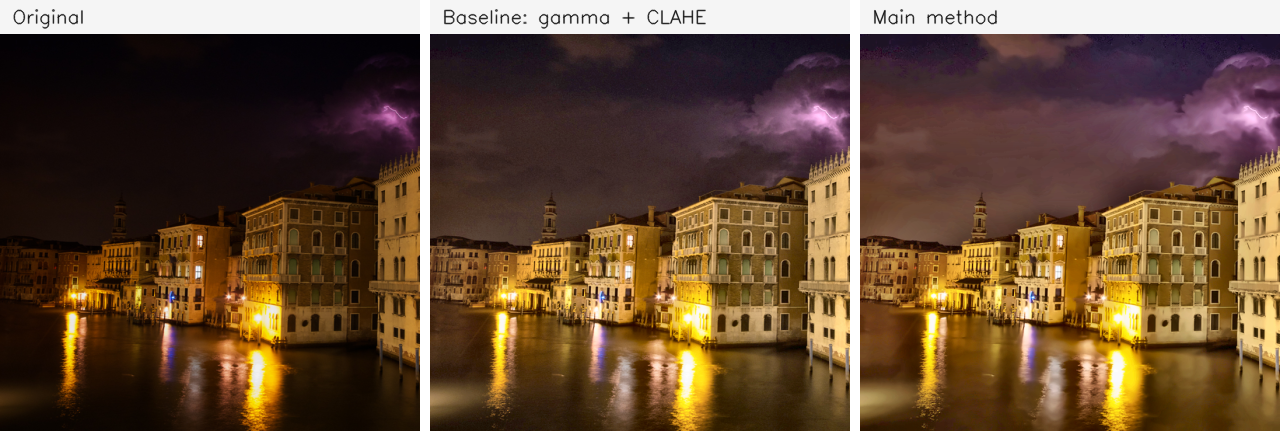
\includegraphics[width=\linewidth]{1_comparison.png}
  \caption{Result for 1.bmp.}
  \label{fig:result1}
\end{figure}

\begin{figure}[H]
  \centering
  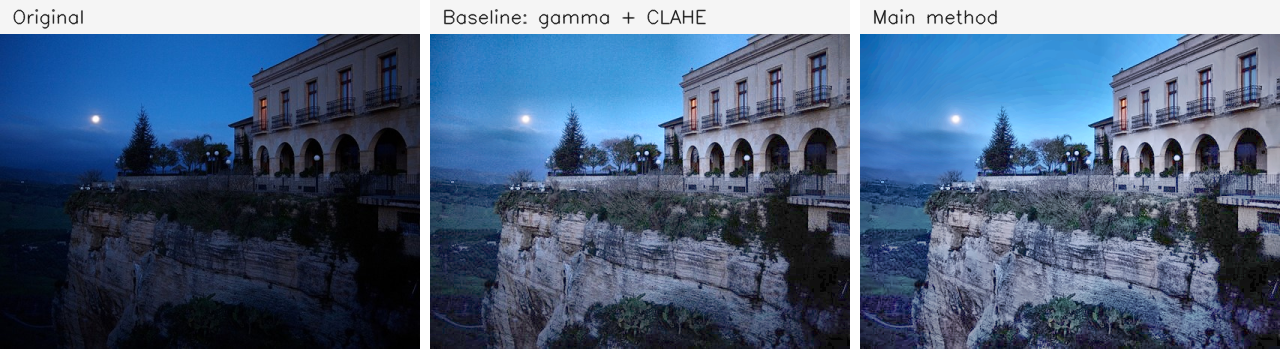
\includegraphics[width=\linewidth]{2_comparison.png}
  \caption{Result for 2.bmp.}
  \label{fig:result2}
\end{figure}

\begin{figure}[H]
  \centering
  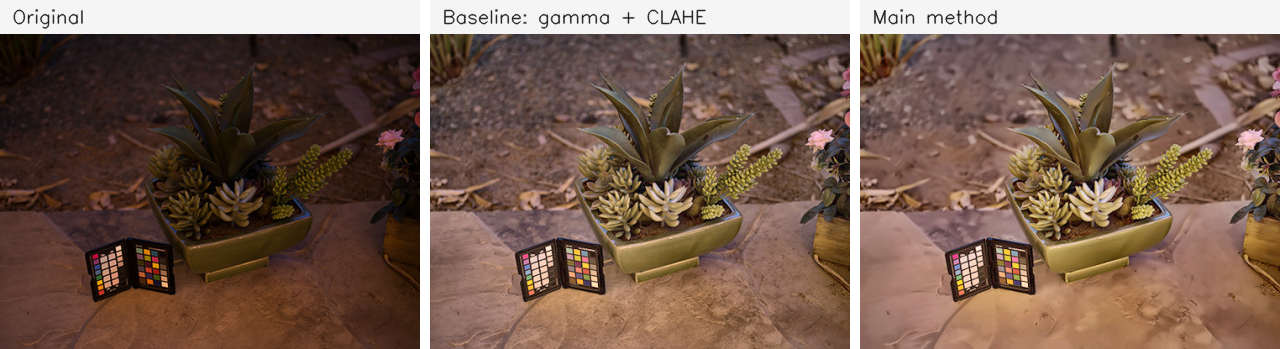
\includegraphics[width=\linewidth]{3_comparison.png}
  \caption{Result for 3.bmp.}
  \label{fig:result3}
\end{figure}

\begin{figure}[H]
  \centering
  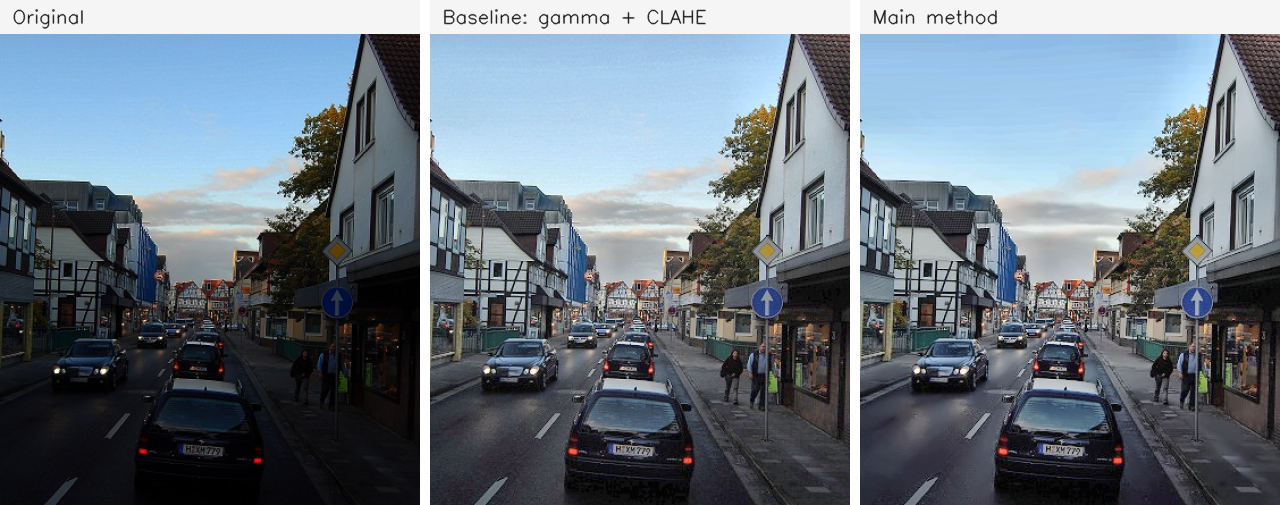
\includegraphics[width=\linewidth]{4_comparison.png}
  \caption{Result for 4.bmp.}
  \label{fig:result4}
\end{figure}

\begin{figure}[H]
  \centering
  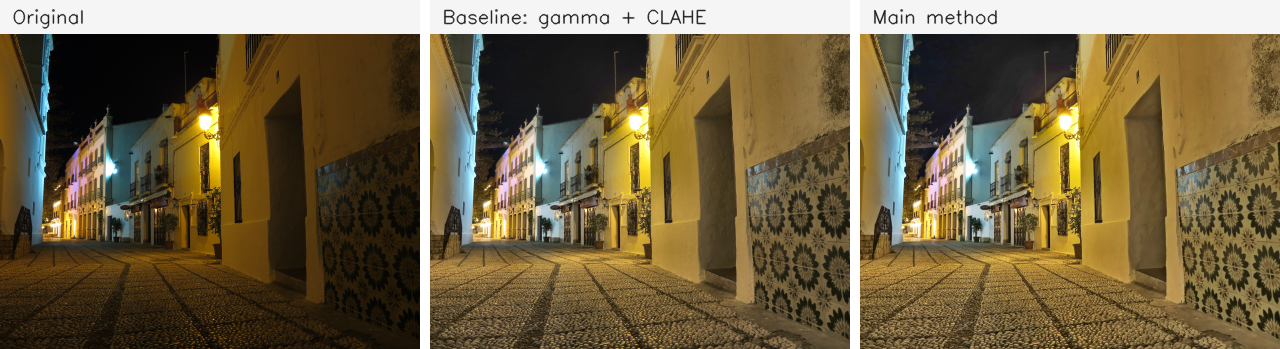
\includegraphics[width=\linewidth]{5_comparison.png}
  \caption{Result for 5.bmp.}
  \label{fig:result5}
\end{figure}

\begin{figure}[H]
  \centering
  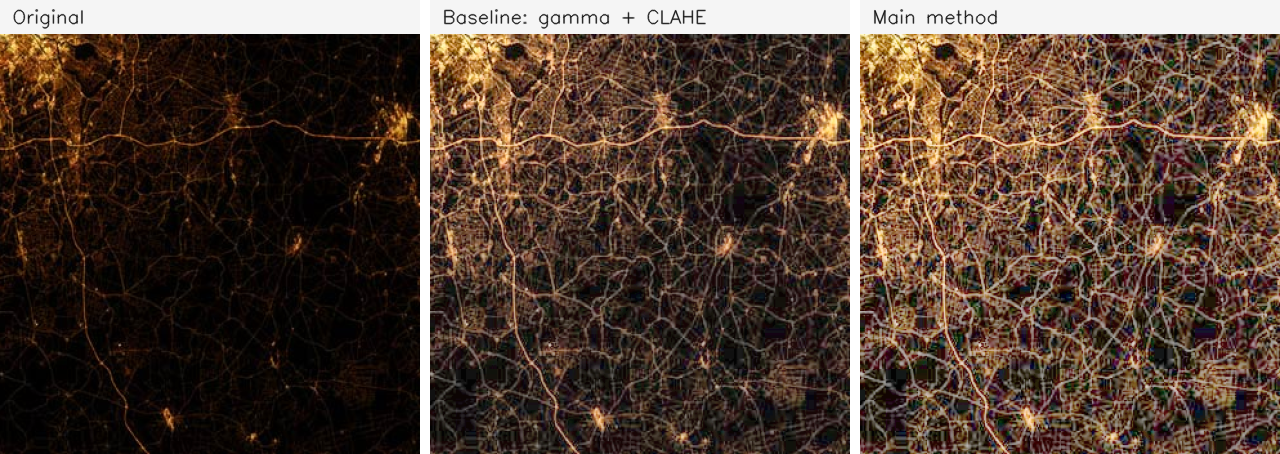
\includegraphics[width=\linewidth]{6_comparison.png}
  \caption{Result for 6.bmp.}
  \label{fig:result6}
\end{figure}

\begin{figure}[H]
  \centering
  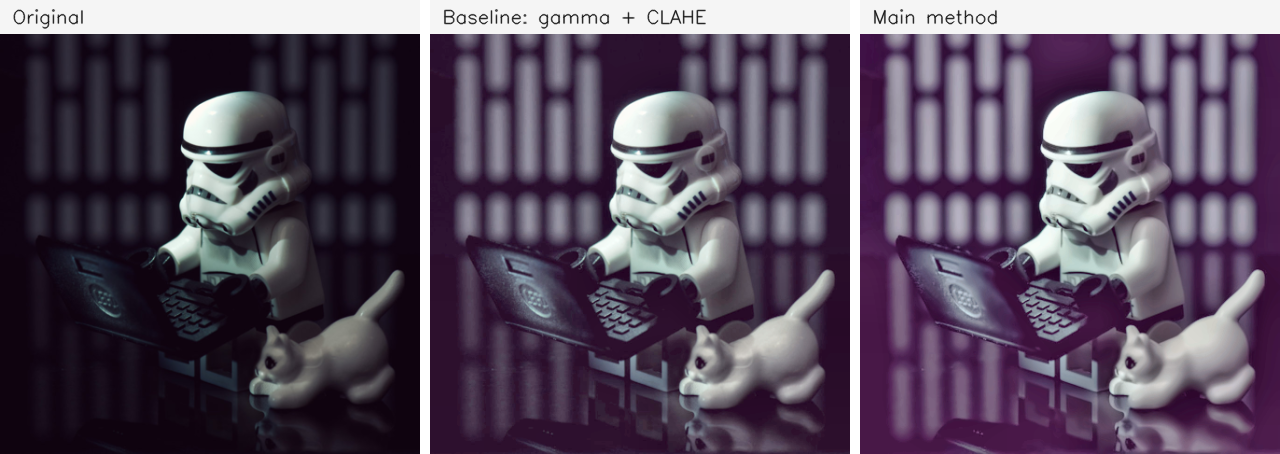
\includegraphics[width=\linewidth]{7_comparison.png}
  \caption{Result for 7.bmp.}
  \label{fig:result7}
\end{figure}

\begin{figure}[H]
  \centering
  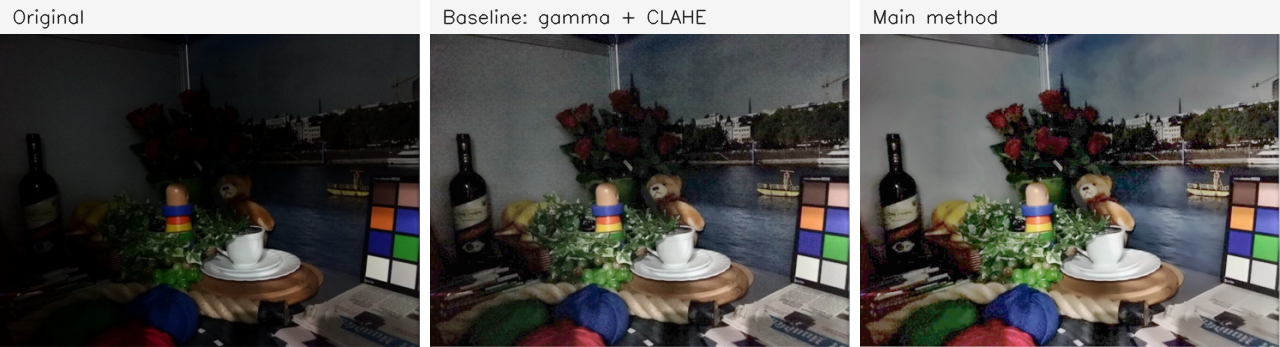
\includegraphics[width=\linewidth]{8_comparison.png}
  \caption{Result for 8.bmp.}
  \label{fig:result8}
\end{figure}

\begin{figure}[H]
  \centering
  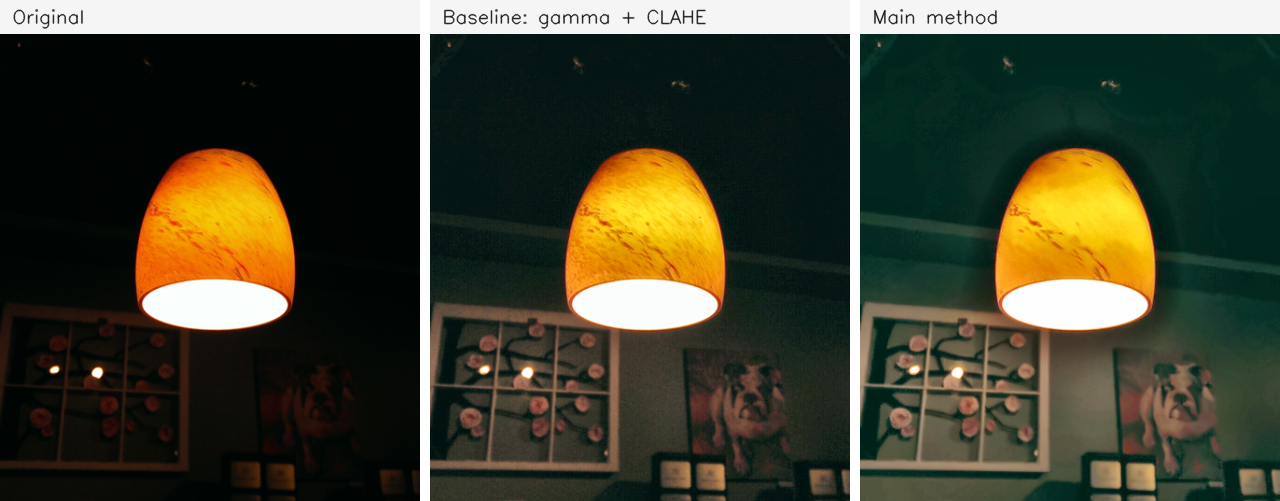
\includegraphics[width=\linewidth]{9_comparison.png}
  \caption{Result for 9.bmp.}
  \label{fig:result9}
\end{figure}

\begin{figure}[H]
  \centering
  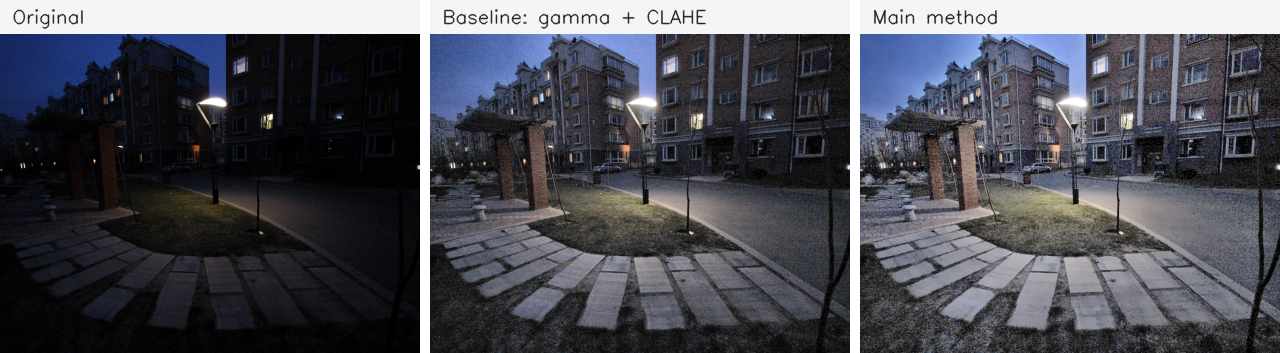
\includegraphics[width=\linewidth]{10_comparison.png}
  \caption{Result for 10.bmp.}
  \label{fig:result10}
\end{figure}

\section{Discussion}

The main method improves visibility in all ten images. Compared with the originals, the enhanced outputs have higher mean luminance and higher entropy, so dark scene details become easier to inspect. The baseline already provides a strong improvement, but the main method usually gives additional illumination correction and stronger shadow recovery.

The method is intentionally conservative. Aggressive illumination division can create over-exposure, color shifts, and strong noise amplification. Therefore, the final implementation uses a small illumination correction strength and blends the corrected image with the gamma-corrected result. This keeps highlights more stable and avoids overly artificial colors.

One difficult case is image 6.bmp, which contains dense bright line structures on a dark background. Enhancement increases visibility but also amplifies high-frequency texture and noise. This is a common tradeoff in low-light enhancement: making hidden details visible can also make unwanted noise more visible. A stronger denoising or structure-aware illumination solver could reduce this artifact, but that would increase implementation complexity.

\section{Conclusion}

This project implements a complete low-light enhancement pipeline for all provided images. The final method combines adaptive gamma correction, denoising, LIME-style illumination estimation, and CLAHE. It is lightweight, reproducible, and does not require paired training data. The results show clear visibility improvements across the full dataset, while the remaining artifacts mainly come from the intrinsic tradeoff between shadow enhancement and noise amplification.

\bibliographystyle{ieeetr}
\bibliography{references}

\end{document}
